% NutraSmart data-flow diagram -- version 01.
%
% Shows how data moves through the NutraSmart program: from the four user
% inputs (food photo, face video, chat message, Google sign-in) through the
% browser UI, CloudFront, the FastAPI edge, the user's regional S3 bucket, the
% regional AgentCore runtime and Bedrock, down to the five outputs the user
% receives. Grounded in the code on branch feature/w360-full as of 2026-10-21:
%   maitribot/client/src/{api.js,App.jsx,FaceScanModal.jsx,DashboardPanel.jsx}
%   backend/app/{main.py,auth.py,regions.py,agent_client.py,config.py}
%   backend/app/routes/{upload,analyze,facescan,chat,meals}.py
%   backend/agent/app/nutrasmart_agent/main.py
%   backend/agent/app/nutrasmart_agent/food_scan/{analysis,services,settings}.py
%   backend/agent/app/nutrasmart_agent/face_scan_biomarkers/{analysis,services,settings}.py
%   documents/DATA_RESIDENCY.md
%
% Layout (top to bottom):
%   1. inputs band       -- food photo, face video, chat message, Google ID token
%   2. browser           -- maitribot/client (React); sends JSON to CloudFront,
%                           PUTs files straight into the regional bucket
%   3. edge              -- CloudFront -> FastAPI edge (ECS Fargate, ap-south-1)
%   4. data region       -- regional S3 bucket (data row, above its consumers),
%                           AgentCore runtime with its four actions, Bedrock,
%                           model stores
%   5. outputs band      -- what comes back to the browser
%
% Simplifications: responses are drawn from the component that produces them
% to the outputs band; in reality every response travels back along the request
% path (agent -> edge -> CloudFront -> browser). The /meals CRUD routes and the
% weekly-summary routes exist on the edge but the current maitribot client only
% calls presign, analyze, facescan/analyze, chat and nutrition/summary.
%
% Abbreviations:
%   uid   = user id derived from the Google e-mail (@ -> _at_, . -> _)
%   ts    = UTC timestamp YYYYMMDDTHHMMSSZ
%   rPPG  = remote photoplethysmography (pulse from skin colour)
%   rBCG  = remote ballistocardiography (pulse from head motion)
%   HR    = heart rate, BP = blood pressure, SpO2 = blood oxygen saturation
%
% Build: pdflatex data-flow-diagram.tex
\documentclass[tikz,border=12pt]{standalone}
\usepackage[T1]{fontenc}
\usepackage{amsmath,amssymb}
\usetikzlibrary{arrows.meta,positioning,fit,backgrounds,calc}

% ---- Palette: one colour per node role, defined once --------------------
\definecolor{inputc}{RGB}{33,102,172}   % external inputs
\definecolor{procc}{RGB}{64,64,64}      % processing stages, arrows
\definecolor{llmc}{RGB}{118,42,131}     % LLM (Bedrock)
\definecolor{datac}{RGB}{1,133,113}     % data stores
\definecolor{outc}{RGB}{178,24,43}      % final outputs
\definecolor{regionc}{RGB}{1,133,113}   % data-region band

\tikzset{
  font=\sffamily\small,
  >={Stealth[length=2.4mm]},
  flow/.style={->, thick, draw=procc},
  both/.style={<->, thick, draw=procc},
  lbl/.style={font=\sffamily\tiny, text=procc, align=left, inner sep=1.5pt},
  box/.style={draw, thick, rounded corners=3pt, minimum height=9mm,
              minimum width=22mm, align=center},
  input/.style={box, draw=inputc, fill=inputc!8, text width=30mm,
                minimum height=12mm},
  process/.style={box, draw=procc, fill=procc!6},
  action/.style={process, text width=35mm, minimum height=20mm},
  llm/.style={box, draw=llmc, fill=llmc!8, text width=32mm, minimum height=13mm},
  data/.style={box, draw=datac, fill=datac!8, rounded corners=9pt,
               minimum width=20mm},
  output/.style={box, draw=outc, fill=outc!8, text width=32mm, minimum height=14mm},
  band/.style={draw=#1!60, dashed, rounded corners=6pt, fill=#1!3,
               inner sep=10pt},
  bandlabel/.style={font=\sffamily\bfseries\footnotesize, text=#1,
                    anchor=south west},
}

% ---- Text helpers ----------------------------------------------------------
\newcommand{\sub}{\sffamily\scriptsize}
\newcommand{\key}{\ttfamily\tiny}

\begin{document}
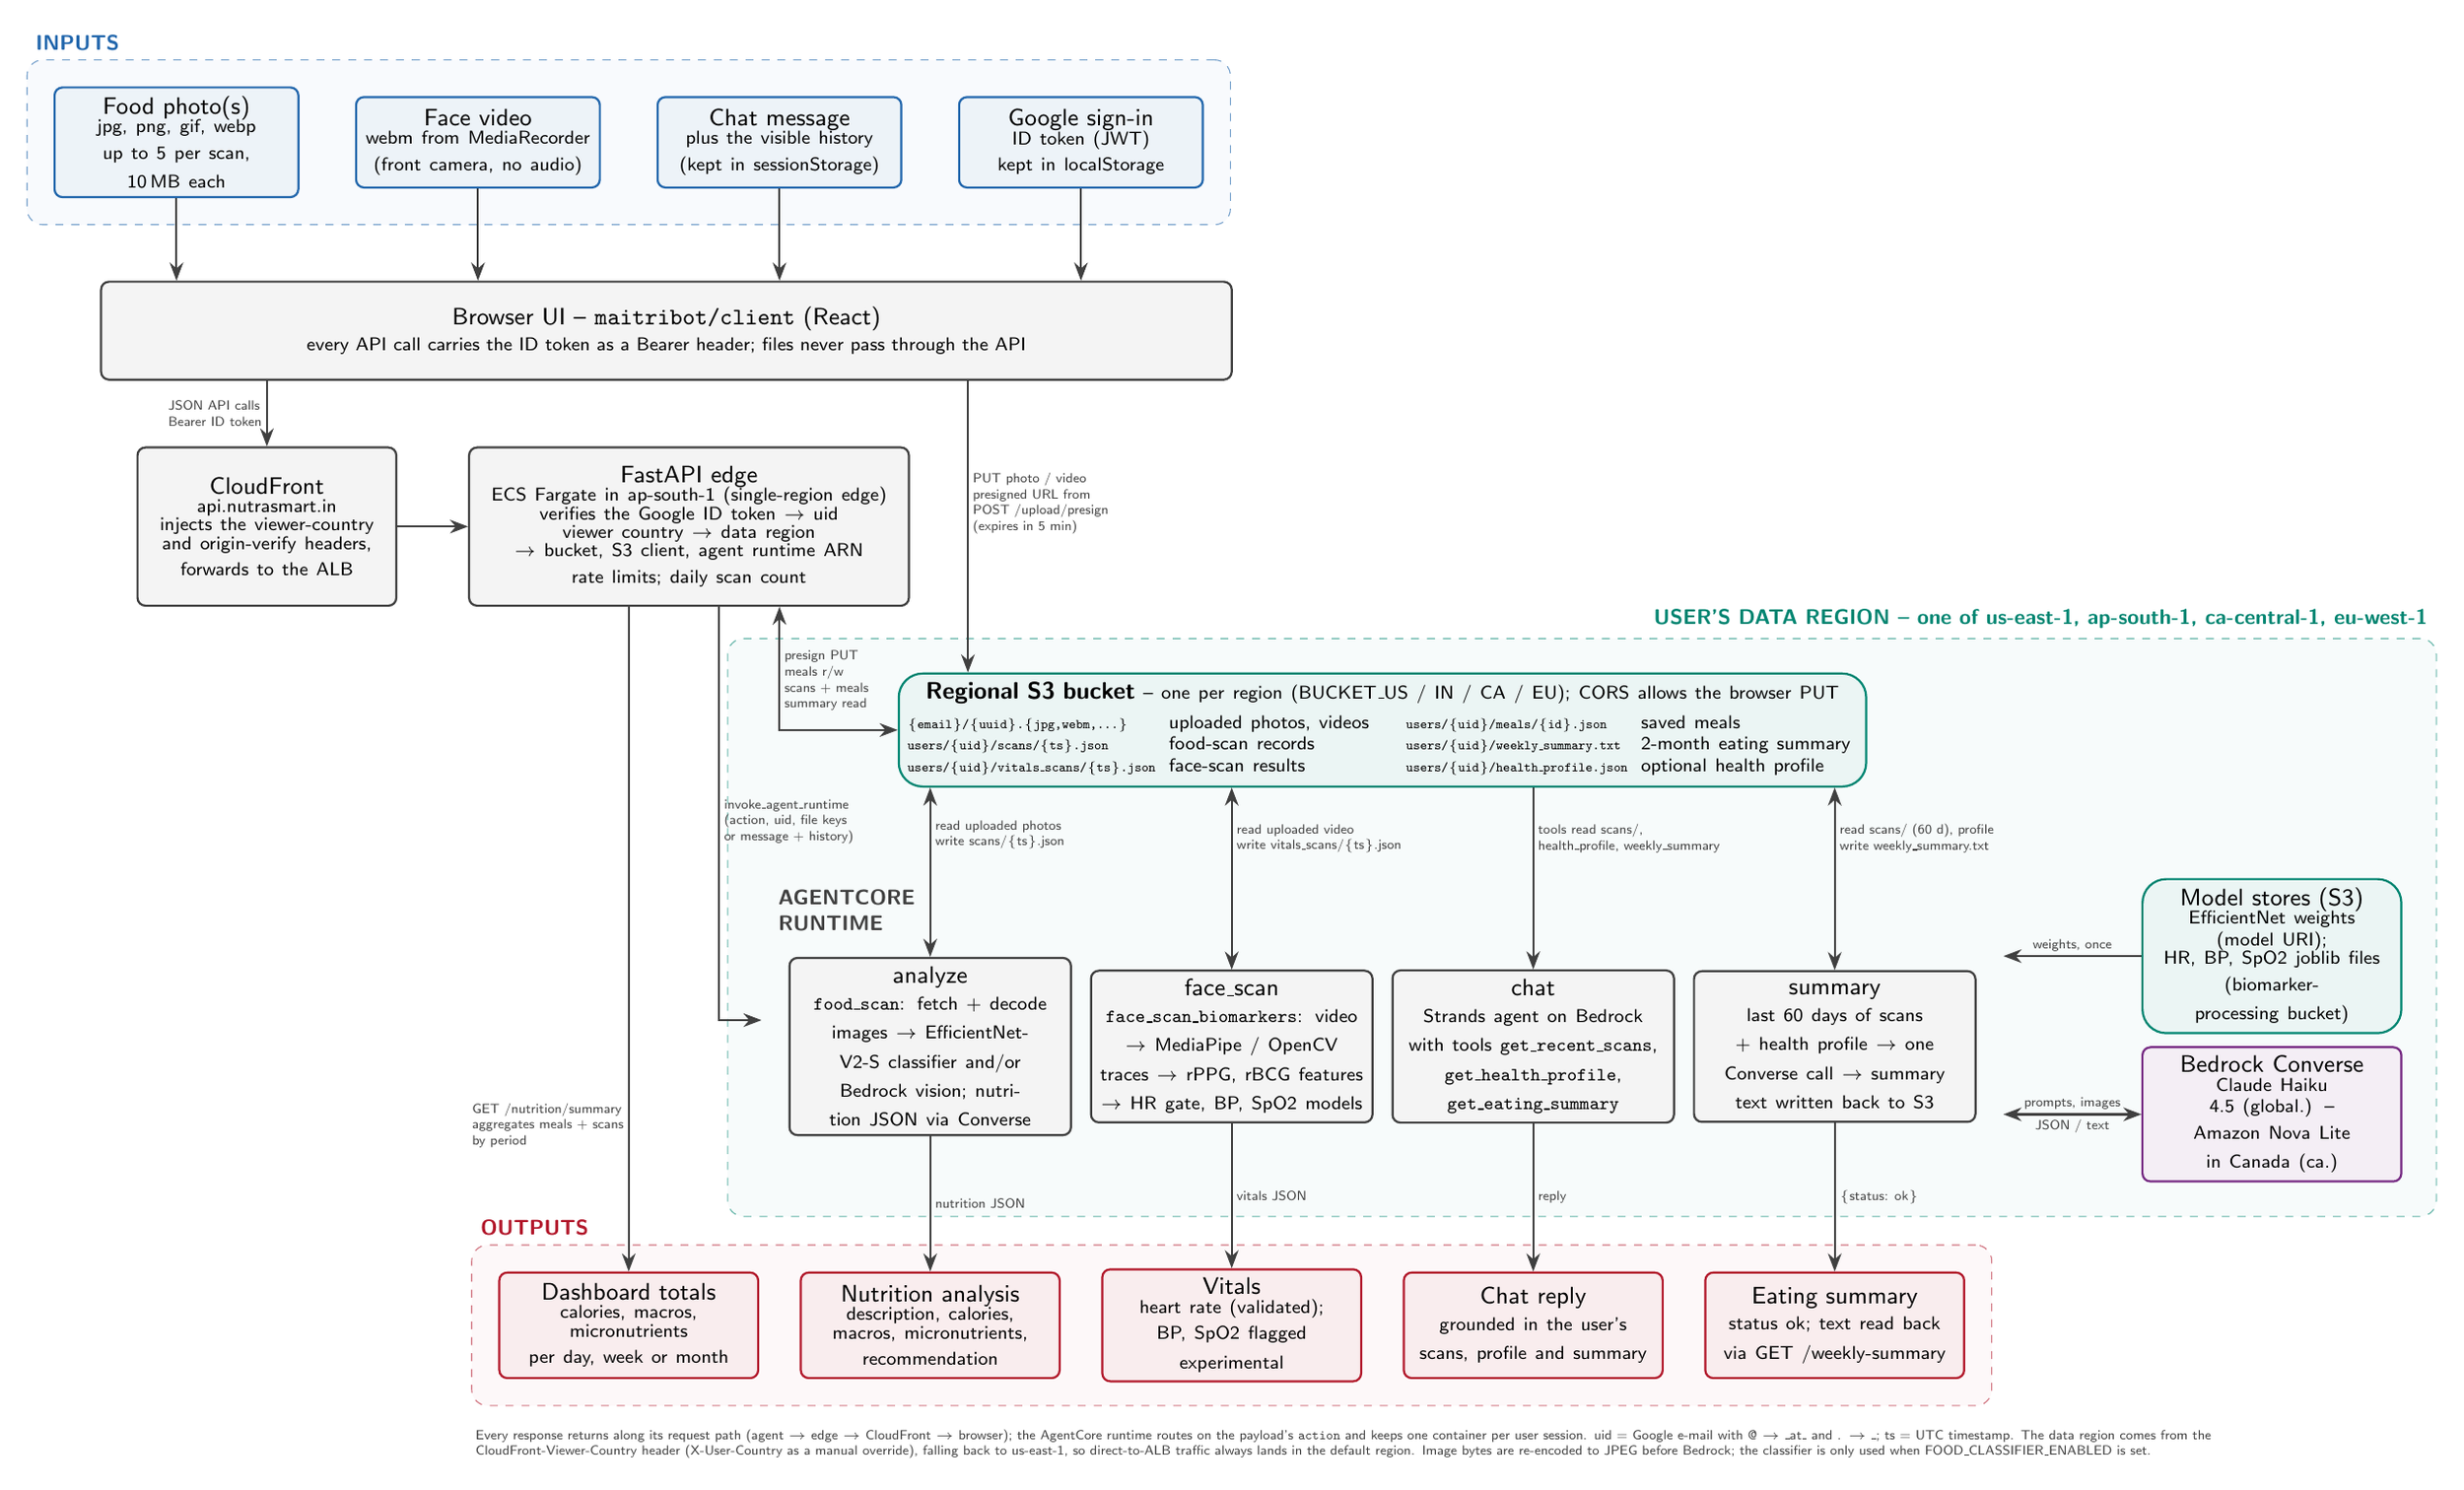
\begin{tikzpicture}

  % ---------------- Inputs (top) ----------------
  \node[input] (inphoto) at (0,0)  {Food photo(s)\\[-1pt]\sub jpg, png, gif, webp\\[-1pt]\sub up to 5 per scan, 10\,MB each};
  \node[input] (invideo) at (4,0)  {Face video\\[-1pt]\sub webm from MediaRecorder\\[-1pt]\sub (front camera, no audio)};
  \node[input] (inchat)  at (8,0)  {Chat message\\[-1pt]\sub plus the visible history\\[-1pt]\sub (kept in sessionStorage)};
  \node[input] (intoken) at (12,0) {Google sign-in\\[-1pt]\sub ID token (JWT)\\[-1pt]\sub kept in localStorage};

  % ---------------- Browser ----------------
  \node[process, minimum width=150mm, minimum height=13mm] (browser) at (6.5,-2.5)
    {Browser UI -- \texttt{maitribot/client} (React)\\[-1pt]
     \sub every API call carries the ID token as a Bearer header; files never pass through the API};

  % ---------------- Edge row ----------------
  \node[process, text width=32mm, minimum height=21mm] (cf) at (1.2,-5.1)
    {CloudFront\\[-1pt]\sub api.nutrasmart.in\\[-1pt]\sub injects the viewer-country\\[-1pt]\sub and origin-verify headers,\\[-1pt]\sub forwards to the ALB};
  \node[process, text width=56mm, minimum height=21mm] (edge) at (6.8,-5.1)
    {FastAPI edge\\[-1pt]
     \sub ECS Fargate in ap-south-1 (single-region edge)\\[-1pt]
     \sub verifies the Google ID token $\to$ uid\\[-1pt]
     \sub viewer country $\to$ data region\\[-1pt]
     \sub $\to$ bucket, S3 client, agent runtime ARN\\[-1pt]
     \sub rate limits; daily scan count};

  % ---------------- Regional S3 bucket (data row, above its consumers) ----------------
  \node[data, text width=126mm, align=left] (s3) at (16,-7.8) {%
    \centering\textbf{Regional S3 bucket} \sub -- one per region (BUCKET\_US / IN / CA / EU); CORS allows the browser PUT\\[3pt]
    \begin{tabular}{@{}l@{\hspace{5pt}}l@{\hspace{14pt}}l@{\hspace{5pt}}l@{}}
      \key \{email\}/\{uuid\}.\{jpg,webm,...\} & \sub uploaded photos, videos &
      \key users/\{uid\}/meals/\{id\}.json     & \sub saved meals \\
      \key users/\{uid\}/scans/\{ts\}.json     & \sub food-scan records &
      \key users/\{uid\}/weekly\_summary.txt   & \sub 2-month eating summary \\
      \key users/\{uid\}/vitals\_scans/\{ts\}.json & \sub face-scan results &
      \key users/\{uid\}/health\_profile.json  & \sub optional health profile \\
    \end{tabular}};

  % ---------------- AgentCore runtime: four actions ----------------
  \node[action] (analyze) at (10,-12.0)
    {analyze\\[-1pt]\sub \texttt{food\_scan}: fetch + decode images $\to$ EfficientNet-V2-S classifier and/or Bedrock vision; nutrition JSON via Converse};
  \node[action] (facescan) at (14,-12.0)
    {face\_scan\\[-1pt]\sub \texttt{face\_scan\_biomarkers}: video $\to$ MediaPipe / OpenCV traces $\to$ rPPG, rBCG features $\to$ HR gate, BP, SpO2 models};
  \node[action] (chat) at (18,-12.0)
    {chat\\[-1pt]\sub Strands agent on Bedrock with tools \texttt{get\_recent\_scans}, \texttt{get\_health\_profile}, \texttt{get\_eating\_summary}};
  \node[action] (summary) at (22,-12.0)
    {summary\\[-1pt]\sub last 60 days of scans + health profile $\to$ one Converse call $\to$ summary text written back to S3};

  \begin{scope}[on background layer]
    \coordinate (agentpad) at ($(analyze.north west)+(0,0.7)$);
    \node[band=procc, inner sep=3.5mm] (agent) [fit=(analyze)(summary)(agentpad)] {};
  \end{scope}
  \node[bandlabel=procc, anchor=north west, align=left] at ($(agent.north west)+(0.1,-0.05)$) {AGENTCORE\\RUNTIME};

  % ---------------- Bedrock and model stores (right of the runtime) ----------------
  \node[data, text width=32mm, minimum height=13mm] (models) at (27.8,-10.8)
    {Model stores (S3)\\[-1pt]\sub EfficientNet weights (model URI);\\[-1pt]\sub HR, BP, SpO2 joblib files\\[-1pt]\sub (biomarker-processing bucket)};
  \node[llm] (bedrock) at (27.8,-12.9)
    {Bedrock Converse\\[-1pt]\sub Claude Haiku 4.5 (global.) --\\[-1pt]\sub Amazon Nova Lite in Canada (ca.)};

  \begin{scope}[on background layer]
    \node[band=regionc, inner sep=4.5mm] (region) [fit=(s3)(agent)(models)(bedrock)] {};
  \end{scope}
  \node[bandlabel=regionc, anchor=south east] at (region.north east)
    {USER'S DATA REGION -- one of us-east-1, ap-south-1, ca-central-1, eu-west-1};

  % ---------------- Outputs (bottom) ----------------
  \node[output] (outdash) at (6.0,-15.7)
    {Dashboard totals\\[-1pt]\sub calories, macros,\\[-1pt]\sub micronutrients\\[-1pt]\sub per day, week or month};
  \node[output] (outfood) at (10,-15.7)
    {Nutrition analysis\\[-1pt]\sub description, calories,\\[-1pt]\sub macros, micronutrients,\\[-1pt]\sub recommendation};
  \node[output] (outvitals) at (14,-15.7)
    {Vitals\\[-1pt]\sub heart rate (validated);\\[-1pt]\sub BP, SpO2 flagged experimental};
  \node[output] (outchat) at (18,-15.7)
    {Chat reply\\[-1pt]\sub grounded in the user's scans, profile and summary};
  \node[output] (outsummary) at (22,-15.7)
    {Eating summary\\[-1pt]\sub status ok; text read back via GET /weekly-summary};

  % ---------------- Edges ----------------
  % inputs -> browser
  \foreach \n in {inphoto,invideo,inchat,intoken} {
    \draw[flow] (\n) -- (\n |- browser.north);
  }

  % browser -> CloudFront -> edge
  \draw[flow] (browser.south -| cf.north) -- (cf.north)
    node[lbl, midway, left] {JSON API calls\\Bearer ID token};
  \draw[flow] (cf) -- (edge);

  % browser -> regional bucket (direct PUT with a presigned URL)
  \draw[flow] (browser.south -| 10.5,0) -- (s3.north -| 10.5,0)
    node[lbl, pos=0.42, right] {PUT photo / video\\presigned URL from\\POST /upload/presign\\(expires in 5 min)};

  % edge -> bucket (edge-side reads and writes)
  \draw[both] ($(edge.south)+(1.2,0)$) |- (s3.west)
    node[lbl, pos=0.3, right] {presign PUT\\meals r/w\\scans + meals\\summary read};

  % edge -> agent runtime
  \draw[flow] ($(edge.south)+(0.4,0)$) |- (agent.west)
    node[lbl, pos=0.26, right] {invoke\_agent\_runtime\\(action, uid, file keys\\or message + history)};

  % edge -> dashboard output
  \draw[flow] ($(edge.south)+(-0.8,0)$) -- (outdash.north)
    node[lbl, pos=0.78, left] {GET /nutrition/summary\\aggregates meals + scans\\by period};

  % actions <-> bucket (per-action reads and writes)
  \draw[both] (analyze.north) -- (analyze.north |- s3.south)
    node[lbl, pos=0.72, right] {read uploaded photos\\write scans/\{ts\}.json};
  \draw[both] (facescan.north) -- (facescan.north |- s3.south)
    node[lbl, pos=0.72, right] {read uploaded video\\write vitals\_scans/\{ts\}.json};
  \draw[flow, <-] (chat.north) -- (chat.north |- s3.south)
    node[lbl, pos=0.72, right] {tools read scans/,\\health\_profile, weekly\_summary};
  \draw[both] (summary.north) -- (summary.north |- s3.south)
    node[lbl, pos=0.72, right] {read scans/ (60 d), profile\\write weekly\_summary.txt};

  % model stores -> runtime, runtime <-> Bedrock
  \draw[flow] (models.west) -- (agent.east |- models.west)
    node[lbl, midway, above] {weights, once};
  \draw[both] (agent.east |- bedrock.west) -- (bedrock.west)
    node[lbl, midway, above] {prompts, images}
    node[lbl, midway, below] {JSON / text};

  % actions -> outputs
  \draw[flow] (analyze) -- (outfood)   node[lbl, midway, right] {nutrition JSON};
  \draw[flow] (facescan) -- (outvitals) node[lbl, midway, right] {vitals JSON};
  \draw[flow] (chat) -- (outchat)       node[lbl, midway, right] {reply};
  \draw[flow] (summary) -- (outsummary) node[lbl, midway, right] {\{status: ok\}};

  % ---------------- Bands ----------------
  \begin{scope}[on background layer]
    \node[band=inputc, fit=(inphoto)(intoken)] (inband) {};
    \node[band=outc, fit=(outdash)(outsummary)] (outband) {};
  \end{scope}
  \node[bandlabel=inputc] at (inband.north west) {INPUTS};
  \node[bandlabel=outc] at (outband.north west) {OUTPUTS};

  % ---------------- Footnote ----------------
  \node[lbl, anchor=north west, text width=240mm] at ($(outband.south west)+(0,-0.25)$)
    {Every response returns along its request path (agent $\to$ edge $\to$ CloudFront $\to$ browser); the AgentCore runtime routes on the payload's \texttt{action} and keeps one container per user session.
     uid = Google e-mail with @ $\to$ \_at\_ and . $\to$ \_; ts = UTC timestamp.
     The data region comes from the CloudFront-Viewer-Country header (X-User-Country as a manual override), falling back to us-east-1,
     so direct-to-ALB traffic always lands in the default region.
     Image bytes are re-encoded to JPEG before Bedrock; the classifier is only used when FOOD\_CLASSIFIER\_ENABLED is set.};

\end{tikzpicture}
\end{document}
